\documentclass[aspectratio=169, 11pt]{beamer}

\usepackage[T1]{fontenc}
\usepackage[utf8]{inputenc}
\usepackage{helvet}
\renewcommand{\familydefault}{\sfdefault}
\usepackage{xcolor}
\usepackage{tikz}
\usetikzlibrary{arrows.meta, positioning, fit, calc, shapes.geometric}
\usepackage{booktabs}
\usepackage{microtype}

\definecolor{kblue}{HTML}{00539F}
\definecolor{kbluedark}{HTML}{003D7A}
\definecolor{kbluelight}{HTML}{E8F2FB}
\definecolor{kbluepale}{HTML}{F4F8FC}
\definecolor{kvideogray}{HTML}{C8D0D8}
\definecolor{kscreenbg}{HTML}{EEF2F7}
\definecolor{korange}{HTML}{E87722}
\definecolor{kgreen}{HTML}{2E8B57}
\definecolor{kgray}{HTML}{6C757D}
\definecolor{klightgray}{HTML}{F0F2F4}

\usetheme{default}
\setbeamercolor{background canvas}{bg=white}
\setbeamercolor{frametitle}{fg=white, bg=kblue}
\setbeamerfont{frametitle}{size=\large, series=\bfseries, family=\sffamily}
\setbeamertemplate{navigation symbols}{}
\setbeamertemplate{footline}{%
  \hfill\tiny\color{kgray}\insertframenumber\hspace{6pt}\vspace{4pt}%
}
\setbeamertemplate{frametitle}{%
  \begin{beamercolorbox}[wd=\paperwidth, ht=0.65cm, dp=0.15cm, leftskip=0.4cm]{frametitle}%
    \usebeamerfont{frametitle}\insertframetitle%
  \end{beamercolorbox}%
}

\tikzset{
  farrow/.style={-{Stealth[length=4pt, width=3pt]}, kgray, line width=0.5pt},
}

\begin{document}

{
\setbeamercolor{background canvas}{bg=kbluedark}
\setbeamertemplate{footline}{}
\begin{frame}
\begin{tikzpicture}[remember picture, overlay]
  \node[anchor=north west, font=\fontsize{22}{26}\selectfont\sffamily\bfseries, text=white]
    at ($(current page.north west)+(1.0,-1.2)$) {User Study --- Trust and Avatar Perception};
  \node[anchor=north west, font=\large\sffamily, text=white!75]
    at ($(current page.north west)+(1.0,-2.3)$) {Article Summaries --- Section 2};
  \draw[white!40, line width=0.5pt] ($(current page.north west)+(1.0,-3.0)$)
    -- ($(current page.north west)+(14.0,-3.0)$);
  \node[anchor=north west, font=\small\sffamily, text=white!80]
    at ($(current page.north west)+(1.0,-3.4)$) {McKnight \& Chervany 2001 \textbullet{} Mayer et al.\ 1995 \textbullet{} Bartneck et al.\ 2009 \textbullet{} Ho \& MacDorman 2010 \textbullet{} Canales et al.\ 2024 \textbullet{} Alipour et al.\ 2025};
  \node[anchor=north west, font=\small\sffamily, text=white!80]
    at ($(current page.north west)+(1.0,-4.1)$) {Nowak \& Biocca 2003 \textbullet{} Nowak \& Rauh 2005 \textbullet{} Weidner et al.\ 2023 \textbullet{} Kuffner dos Anjos \& Pereira 2024};
  \node[anchor=north west, font=\small\sffamily, text=white!80]
    at ($(current page.north west)+(1.0,-4.8)$) {Alimardani et al.\ 2024 \textbullet{} Dubosc et al.\ 2025 \textbullet{} Tao et al.\ 2025 \textbullet{} Cihodaru-\c{S}tefanache \& Podina 2025 \textbullet{} Wallraven et al.\ 2008};
  \node[anchor=south west, font=\small\sffamily, text=white!60]
    at ($(current page.south west)+(1.0,0.5)$)
    {Nidanur G\"unay \quad\textbullet\quad University of Konstanz \quad\textbullet\quad 2026};
\end{tikzpicture}
\end{frame}
}

%% ═══════════════════════════════════════════════════════════════════════════
%% McKnight & Chervany 2001
%% ═══════════════════════════════════════════════════════════════════════════
\begin{frame}{McKnight \& Chervany (2001) \textnormal{\normalsize --- What Trust Means}}
\begin{center}
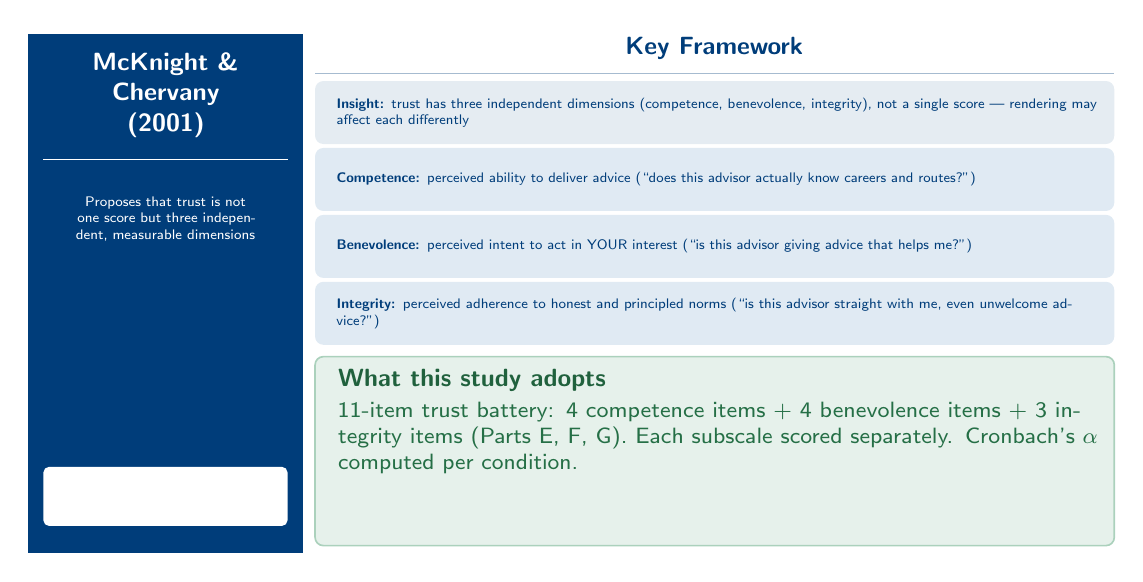
\begin{tikzpicture}[x=1cm, y=1cm]
\fill[kbluedark] (0.0,0.0) rectangle (3.5,6.6);
\node[font=\small\sffamily\bfseries, text=white, align=center, text width=3.1cm]
  at (1.75,5.82) {McKnight \&\\Chervany\\(2001)};
\draw[white!30, line width=0.3pt] (0.2,5.00) -- (3.3,5.00);
\node[font=\tiny\sffamily, text=white!85, align=center, text width=3.0cm]
  at (1.75,4.25) {Proposes that trust is not one score but three independent, measurable dimensions};
\fill[white!20, rounded corners=2pt] (0.2,0.35) rectangle (3.3,1.10);
\node[font=\tiny\sffamily\bfseries, text=white, align=center]
  at (1.75,0.72) {Theoretical\\conceptual typology};
\node[font=\small\sffamily\bfseries\color{kbluedark}] at (8.72,6.42) {Key Framework};
\draw[kbluedark!35, line width=0.3pt] (3.65,6.10) -- (13.8,6.10);
\fill[kbluedark!10, rounded corners=3pt] (3.65,5.20) rectangle (13.8,6.00);
\node[font=\tiny\sffamily\color{kbluedark}, anchor=west, text width=9.65cm]
  at (3.80,5.60) {\textbf{Insight:} trust has three independent dimensions (competence, benevolence, integrity), not a single score --- rendering may affect each differently};
\fill[kblue!12, rounded corners=3pt] (3.65,4.35) rectangle (13.8,5.15);
\node[font=\tiny\sffamily\color{kbluedark}, anchor=west, text width=9.65cm]
  at (3.80,4.75) {\textbf{Competence:} perceived ability to deliver advice (``does this advisor actually know careers and routes?'')};
\fill[kblue!12, rounded corners=3pt] (3.65,3.50) rectangle (13.8,4.30);
\node[font=\tiny\sffamily\color{kbluedark}, anchor=west, text width=9.65cm]
  at (3.80,3.90) {\textbf{Benevolence:} perceived intent to act in YOUR interest (``is this advisor giving advice that helps me?'')};
\fill[kblue!12, rounded corners=3pt] (3.65,2.65) rectangle (13.8,3.45);
\node[font=\tiny\sffamily\color{kbluedark}, anchor=west, text width=9.65cm]
  at (3.80,3.05) {\textbf{Integrity:} perceived adherence to honest and principled norms (``is this advisor straight with me, even unwelcome advice?'')};
\fill[kgreen!12, draw=kgreen!40, rounded corners=3pt, line width=0.6pt]
  (3.65,0.1) rectangle (13.8,2.50);
\node[font=\small\sffamily\bfseries\color{kgreen!70!black}, anchor=west]
  at (3.82,2.20) {What this study adopts};
\node[font=\footnotesize\sffamily\color{kgreen!80!black}, anchor=north west, text width=9.65cm]
  at (3.82,2.05) {11-item trust battery: 4 competence items + 4 benevolence items + 3 integrity items (Parts E, F, G). Each subscale scored separately. Cronbach's $\alpha$ computed per condition.};
\end{tikzpicture}
\end{center}
\end{frame}

%% ═══════════════════════════════════════════════════════════════════════════
%% Mayer, Davis & Schoorman 1995
%% ═══════════════════════════════════════════════════════════════════════════
\begin{frame}{Mayer, Davis \& Schoorman (1995) \textnormal{\normalsize --- Integrative Model of Trust}}
\begin{center}
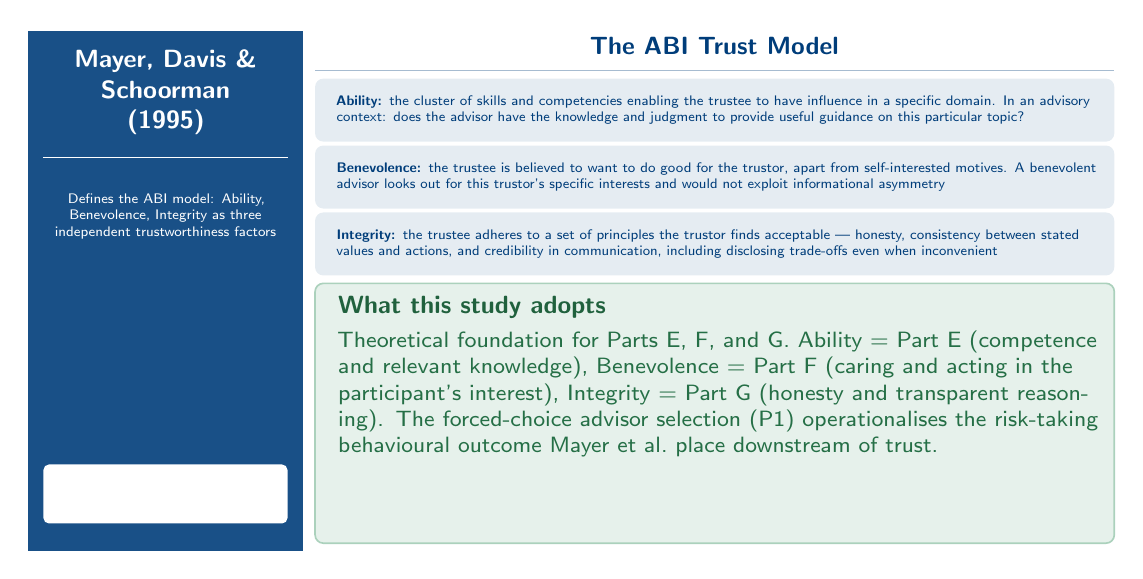
\begin{tikzpicture}[x=1cm, y=1cm]
\fill[kbluedark!90] (0.0,0.0) rectangle (3.5,6.6);
\node[font=\small\sffamily\bfseries, text=white, align=center, text width=3.1cm]
  at (1.75,5.82) {Mayer, Davis \&\\Schoorman\\(1995)};
\draw[white!30, line width=0.3pt] (0.2,5.00) -- (3.3,5.00);
\node[font=\tiny\sffamily, text=white!85, align=center, text width=3.0cm]
  at (1.75,4.25) {Defines the ABI model: Ability, Benevolence, Integrity as three independent trustworthiness factors};
\fill[white!20, rounded corners=2pt] (0.2,0.35) rectangle (3.3,1.10);
\node[font=\tiny\sffamily\bfseries, text=white, align=center]
  at (1.75,0.72) {Theoretical\\integrative review};
\node[font=\small\sffamily\bfseries\color{kbluedark}] at (8.72,6.42) {The ABI Trust Model};
\draw[kbluedark!35, line width=0.3pt] (3.65,6.10) -- (13.8,6.10);
\fill[kbluedark!10, rounded corners=3pt] (3.65,5.20) rectangle (13.8,6.00);
\node[font=\tiny\sffamily\color{kbluedark}, anchor=west, text width=9.65cm]
  at (3.80,5.60) {\textbf{Ability:} the cluster of skills and competencies enabling the trustee to have influence in a specific domain. In an advisory context: does the advisor have the knowledge and judgment to provide useful guidance on this particular topic?};
\fill[kbluedark!10, rounded corners=3pt] (3.65,4.35) rectangle (13.8,5.15);
\node[font=\tiny\sffamily\color{kbluedark}, anchor=west, text width=9.65cm]
  at (3.80,4.75) {\textbf{Benevolence:} the trustee is believed to want to do good for the trustor, apart from self-interested motives. A benevolent advisor looks out for this trustor's specific interests and would not exploit informational asymmetry};
\fill[kbluedark!10, rounded corners=3pt] (3.65,3.50) rectangle (13.8,4.30);
\node[font=\tiny\sffamily\color{kbluedark}, anchor=west, text width=9.65cm]
  at (3.80,3.90) {\textbf{Integrity:} the trustee adheres to a set of principles the trustor finds acceptable --- honesty, consistency between stated values and actions, and credibility in communication, including disclosing trade-offs even when inconvenient};
\fill[kgreen!12, draw=kgreen!40, rounded corners=3pt, line width=0.6pt]
  (3.65,0.1) rectangle (13.8,3.40);
\node[font=\small\sffamily\bfseries\color{kgreen!70!black}, anchor=west]
  at (3.82,3.1) {What this study adopts};
\node[font=\footnotesize\sffamily\color{kgreen!80!black}, anchor=north west, text width=9.65cm]
  at (3.82,2.92) {Theoretical foundation for Parts E, F, and G. Ability = Part E (competence and relevant knowledge), Benevolence = Part F (caring and acting in the participant's interest), Integrity = Part G (honesty and transparent reasoning). The forced-choice advisor selection (P1) operationalises the risk-taking behavioural outcome Mayer et al.\ place downstream of trust.};
\end{tikzpicture}
\end{center}
\end{frame}

%% ═══════════════════════════════════════════════════════════════════════════
%% Bartneck et al. 2009 — Slide 1
%% ═══════════════════════════════════════════════════════════════════════════
\begin{frame}{Bartneck et al. (2009) \textnormal{\normalsize --- Godspeed Questionnaire}}
\begin{center}
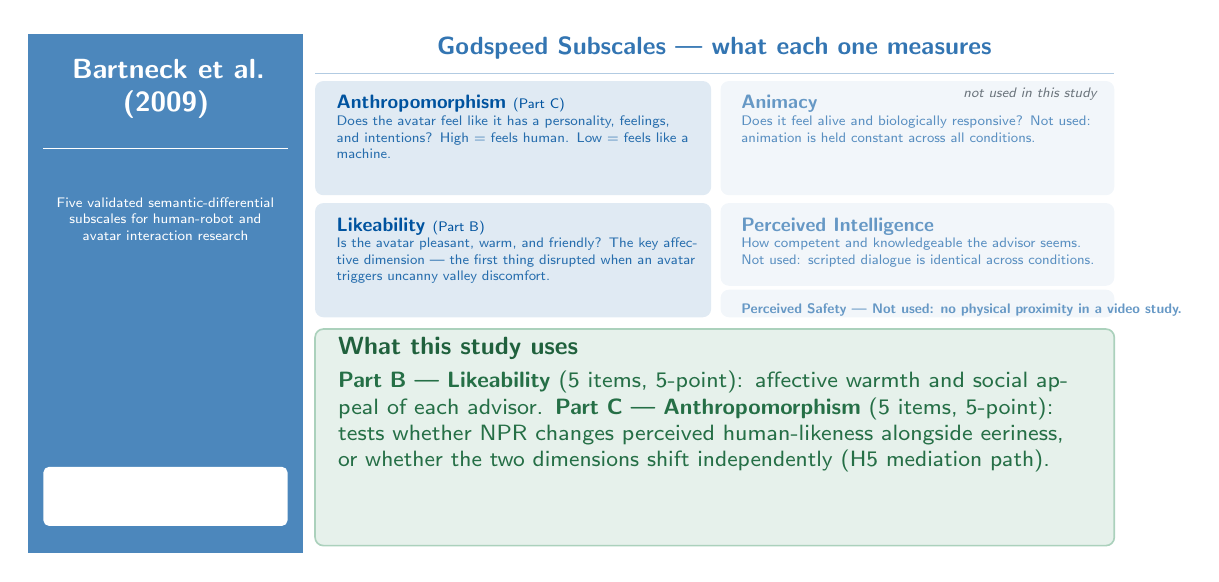
\begin{tikzpicture}[x=1cm, y=1cm]
\fill[kblue!70] (0.0,0.0) rectangle (3.5,6.6);
\node[font=\normalsize\sffamily\bfseries, text=white, align=center, text width=3.1cm]
  at (1.75,5.9) {Bartneck et al.\\(2009)};
\draw[white!30, line width=0.3pt] (0.2,5.15) -- (3.3,5.15);
\node[font=\tiny\sffamily, text=white!85, align=center, text width=3.0cm]
  at (1.75,4.25) {Five validated semantic-differential subscales for human-robot and avatar interaction research};
\fill[white!20, rounded corners=2pt] (0.2,0.35) rectangle (3.3,1.10);
\node[font=\tiny\sffamily\bfseries, text=white, align=center]
  at (1.75,0.72) {Validation study\\n = 156};
\node[font=\small\sffamily\bfseries\color{kblue!80}] at (8.72,6.42) {Godspeed Subscales --- what each one measures};
\draw[kblue!30, line width=0.3pt] (3.65,6.10) -- (13.8,6.10);
\fill[kblue!12, rounded corners=3pt] (3.65,4.55) rectangle (8.68,6.00);
\node[font=\scriptsize\sffamily\bfseries\color{kblue}, anchor=north west] at (3.80,5.94)
  {Anthropomorphism \textnormal{\tiny (Part C)}};
\node[font=\tiny\sffamily\color{kblue!85}, anchor=north west, text width=4.55cm] at (3.80,5.68)
  {Does the avatar feel like it has a personality, feelings, and intentions? High = feels human. Low = feels like a machine.};
\fill[kblue!12, rounded corners=3pt] (3.65,3.00) rectangle (8.68,4.45);
\node[font=\scriptsize\sffamily\bfseries\color{kblue}, anchor=north west] at (3.80,4.39)
  {Likeability \textnormal{\tiny (Part B)}};
\node[font=\tiny\sffamily\color{kblue!85}, anchor=north west, text width=4.55cm] at (3.80,4.13)
  {Is the avatar pleasant, warm, and friendly? The key affective dimension --- the first thing disrupted when an avatar triggers uncanny valley discomfort.};
\fill[kblue!5, rounded corners=3pt] (8.80,4.55) rectangle (13.80,6.00);
\node[font=\scriptsize\sffamily\bfseries\color{kblue!60}, anchor=north west] at (8.94,5.94)
  {Animacy};
\node[font=\tiny\sffamily\color{kblue!65}, anchor=north west, text width=4.55cm] at (8.94,5.68)
  {Does it feel alive and biologically responsive? Not used: animation is held constant across all conditions.};
\fill[kblue!5, rounded corners=3pt] (8.80,3.40) rectangle (13.80,4.45);
\node[font=\scriptsize\sffamily\bfseries\color{kblue!60}, anchor=north west] at (8.94,4.39)
  {Perceived Intelligence};
\node[font=\tiny\sffamily\color{kblue!65}, anchor=north west, text width=4.55cm] at (8.94,4.13)
  {How competent and knowledgeable the advisor seems. Not used: scripted dialogue is identical across conditions.};
\fill[kblue!5, rounded corners=3pt] (8.80,3.00) rectangle (13.80,3.35);
\node[font=\tiny\sffamily\bfseries\color{kblue!60}, anchor=north west] at (8.94,3.30)
  {Perceived Safety --- Not used: no physical proximity in a video study.};
\node[font=\tiny\sffamily\color{kgray}, anchor=north east] at (13.72,6.04)
  {\textit{not used in this study}};
\fill[kgreen!12, draw=kgreen!40, rounded corners=3pt, line width=0.6pt]
  (3.65,0.1) rectangle (13.8,2.85);
\node[font=\small\sffamily\bfseries\color{kgreen!70!black}, anchor=west]
  at (3.82,2.60) {What this study uses};
\node[font=\footnotesize\sffamily\color{kgreen!80!black}, anchor=north west, text width=9.65cm]
  at (3.82,2.44) {\textbf{Part B --- Likeability} (5 items, 5-point): affective warmth and social appeal of each advisor. \textbf{Part C --- Anthropomorphism} (5 items, 5-point): tests whether NPR changes perceived human-likeness alongside eeriness, or whether the two dimensions shift independently (H5 mediation path).};
\end{tikzpicture}
\end{center}
\end{frame}

%% ═══════════════════════════════════════════════════════════════════════════
%% Bartneck et al. 2009 — Slide 2 (exclusion rationale)
%% ═══════════════════════════════════════════════════════════════════════════
\begin{frame}{Bartneck et al. (2009) \textnormal{\normalsize --- Why Only Two Subscales Are Used}}
\begin{center}
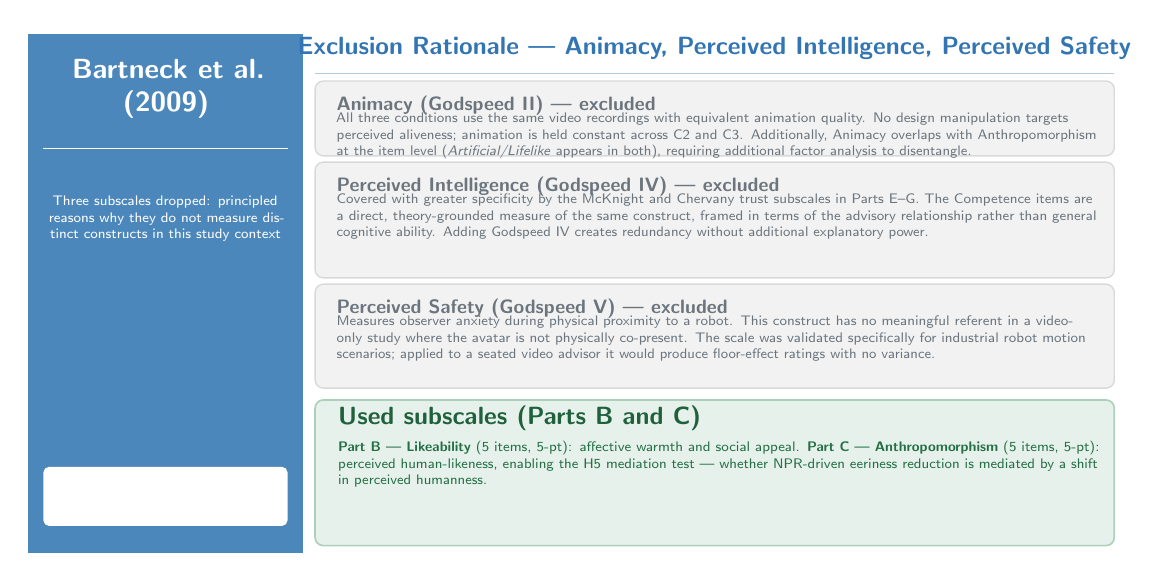
\begin{tikzpicture}[x=1cm, y=1cm]
\fill[kblue!70] (0.0,0.0) rectangle (3.5,6.6);
\node[font=\normalsize\sffamily\bfseries, text=white, align=center, text width=3.1cm]
  at (1.75,5.9) {Bartneck et al.\\(2009)};
\draw[white!30, line width=0.3pt] (0.2,5.15) -- (3.3,5.15);
\node[font=\tiny\sffamily, text=white!85, align=center, text width=3.0cm]
  at (1.75,4.25) {Three subscales dropped: principled reasons why they do not measure distinct constructs in this study context};
\fill[white!20, rounded corners=2pt] (0.2,0.35) rectangle (3.3,1.10);
\node[font=\tiny\sffamily\bfseries, text=white, align=center]
  at (1.75,0.72) {Used:\\Parts B + C only};
\node[font=\small\sffamily\bfseries\color{kblue!80}] at (8.72,6.42) {Exclusion Rationale --- Animacy, Perceived Intelligence, Perceived Safety};
\draw[kblue!30, line width=0.3pt] (3.65,6.10) -- (13.8,6.10);
\fill[gray!10, draw=gray!30, rounded corners=3pt, line width=0.5pt] (3.65,5.05) rectangle (13.8,6.00);
\node[font=\scriptsize\sffamily\bfseries\color{kgray}, anchor=north west] at (3.80,5.94)
  {Animacy (Godspeed II) --- excluded};
\node[font=\tiny\sffamily\color{kgray}, anchor=north west, text width=9.65cm] at (3.80,5.72)
  {All three conditions use the same video recordings with equivalent animation quality. No design manipulation targets perceived aliveness; animation is held constant across C2 and C3. Additionally, Animacy overlaps with Anthropomorphism at the item level (\textit{Artificial/Lifelike} appears in both), requiring additional factor analysis to disentangle.};
\fill[gray!10, draw=gray!30, rounded corners=3pt, line width=0.5pt] (3.65,3.50) rectangle (13.8,4.97);
\node[font=\scriptsize\sffamily\bfseries\color{kgray}, anchor=north west] at (3.80,4.91)
  {Perceived Intelligence (Godspeed IV) --- excluded};
\node[font=\tiny\sffamily\color{kgray}, anchor=north west, text width=9.65cm] at (3.80,4.69)
  {Covered with greater specificity by the McKnight and Chervany trust subscales in Parts E--G. The Competence items are a direct, theory-grounded measure of the same construct, framed in terms of the advisory relationship rather than general cognitive ability. Adding Godspeed IV creates redundancy without additional explanatory power.};
\fill[gray!10, draw=gray!30, rounded corners=3pt, line width=0.5pt] (3.65,2.10) rectangle (13.8,3.42);
\node[font=\scriptsize\sffamily\bfseries\color{kgray}, anchor=north west] at (3.80,3.36)
  {Perceived Safety (Godspeed V) --- excluded};
\node[font=\tiny\sffamily\color{kgray}, anchor=north west, text width=9.65cm] at (3.80,3.14)
  {Measures observer anxiety during physical proximity to a robot. This construct has no meaningful referent in a video-only study where the avatar is not physically co-present. The scale was validated specifically for industrial robot motion scenarios; applied to a seated video advisor it would produce floor-effect ratings with no variance.};
\fill[kgreen!12, draw=kgreen!40, rounded corners=3pt, line width=0.6pt]
  (3.65,0.1) rectangle (13.8,1.95);
\node[font=\small\sffamily\bfseries\color{kgreen!70!black}, anchor=west]
  at (3.82,1.72) {Used subscales (Parts B and C)};
\node[font=\tiny\sffamily\color{kgreen!80!black}, anchor=north west, text width=9.65cm]
  at (3.82,1.55) {\textbf{Part B --- Likeability} (5 items, 5-pt): affective warmth and social appeal. \textbf{Part C --- Anthropomorphism} (5 items, 5-pt): perceived human-likeness, enabling the H5 mediation test --- whether NPR-driven eeriness reduction is mediated by a shift in perceived humanness.};
\end{tikzpicture}
\end{center}
\end{frame}

%% ═══════════════════════════════════════════════════════════════════════════
%% Ho & MacDorman 2010
%% ═══════════════════════════════════════════════════════════════════════════
\begin{frame}{Ho \& MacDorman (2010) \textnormal{\normalsize --- Eeriness Scale}}
\begin{center}
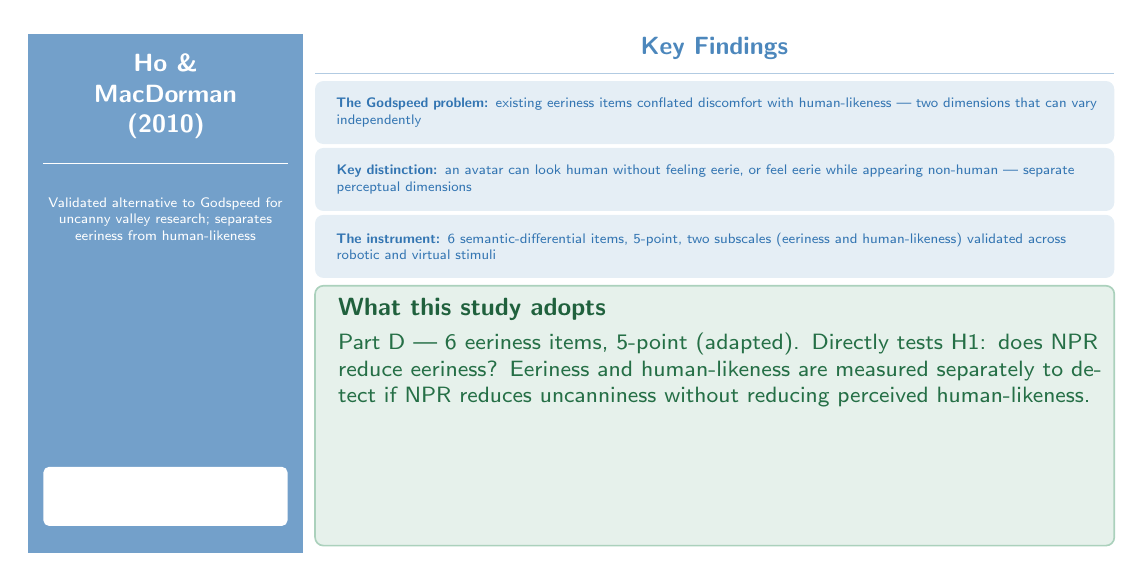
\begin{tikzpicture}[x=1cm, y=1cm]
\fill[kblue!55] (0.0,0.0) rectangle (3.5,6.6);
\node[font=\small\sffamily\bfseries, text=white, align=center, text width=3.1cm]
  at (1.75,5.8) {Ho \&\\MacDorman\\(2010)};
\draw[white!30, line width=0.3pt] (0.2,4.95) -- (3.3,4.95);
\node[font=\tiny\sffamily, text=white!85, align=center, text width=3.0cm]
  at (1.75,4.25) {Validated alternative to Godspeed for uncanny valley research; separates eeriness from human-likeness};
\fill[white!20, rounded corners=2pt] (0.2,0.35) rectangle (3.3,1.10);
\node[font=\tiny\sffamily\bfseries, text=white, align=center]
  at (1.75,0.72) {Validation study\\multiple stimulus types};
\node[font=\small\sffamily\bfseries\color{kblue!70}] at (8.72,6.42) {Key Findings};
\draw[kblue!30, line width=0.3pt] (3.65,6.10) -- (13.8,6.10);
\fill[kblue!10, rounded corners=3pt] (3.65,5.20) rectangle (13.8,6.00);
\node[font=\tiny\sffamily\color{kblue!80}, anchor=west, text width=9.65cm]
  at (3.80,5.60) {\textbf{The Godspeed problem:} existing eeriness items conflated discomfort with human-likeness --- two dimensions that can vary independently};
\fill[kblue!10, rounded corners=3pt] (3.65,4.35) rectangle (13.8,5.15);
\node[font=\tiny\sffamily\color{kblue!80}, anchor=west, text width=9.65cm]
  at (3.80,4.75) {\textbf{Key distinction:} an avatar can look human without feeling eerie, or feel eerie while appearing non-human --- separate perceptual dimensions};
\fill[kblue!10, rounded corners=3pt] (3.65,3.50) rectangle (13.8,4.30);
\node[font=\tiny\sffamily\color{kblue!80}, anchor=west, text width=9.65cm]
  at (3.80,3.90) {\textbf{The instrument:} 6 semantic-differential items, 5-point, two subscales (eeriness and human-likeness) validated across robotic and virtual stimuli};
\fill[kgreen!12, draw=kgreen!40, rounded corners=3pt, line width=0.6pt]
  (3.65,0.1) rectangle (13.8,3.40);
\node[font=\small\sffamily\bfseries\color{kgreen!70!black}, anchor=west]
  at (3.82,3.1) {What this study adopts};
\node[font=\footnotesize\sffamily\color{kgreen!80!black}, anchor=north west, text width=9.65cm]
  at (3.82,2.92) {Part D --- 6 eeriness items, 5-point (adapted). Directly tests H1: does NPR reduce eeriness? Eeriness and human-likeness are measured separately to detect if NPR reduces uncanniness without reducing perceived human-likeness.};
\end{tikzpicture}
\end{center}
\end{frame}

%% ═══════════════════════════════════════════════════════════════════════════
%% Canales et al. 2024
%% ═══════════════════════════════════════════════════════════════════════════
\begin{frame}{Canales, Roble \& Neff (2024) \textnormal{\normalsize --- Avatar Stylisation and Trust}}
\begin{center}
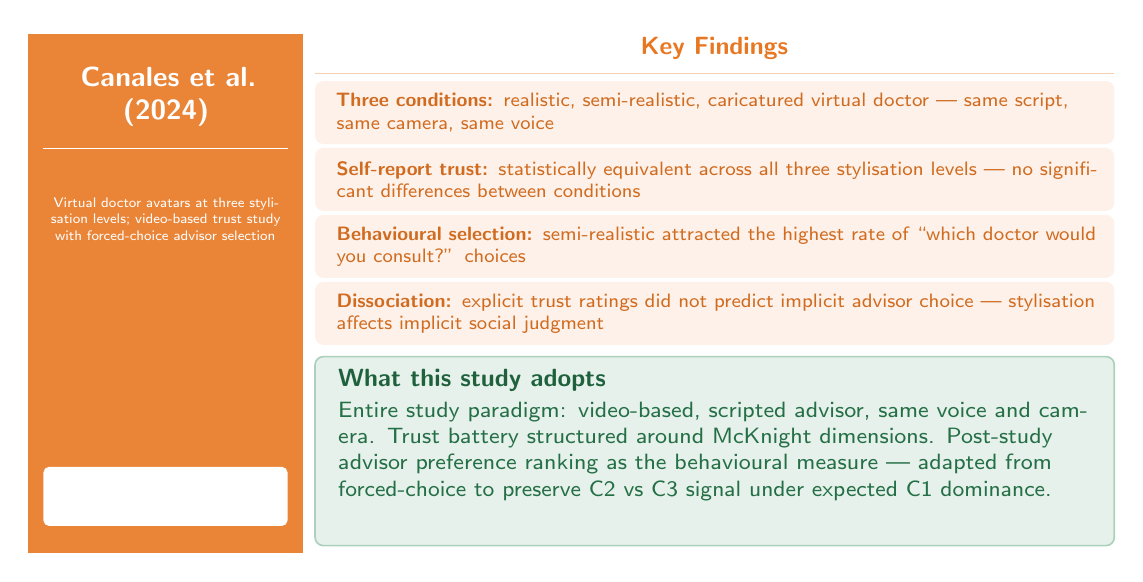
\begin{tikzpicture}[x=1cm, y=1cm]
\fill[korange!90] (0.0,0.0) rectangle (3.5,6.6);
\node[font=\normalsize\sffamily\bfseries, text=white, align=center, text width=3.1cm]
  at (1.75,5.8) {Canales et al.\\(2024)};
\draw[white!30, line width=0.3pt] (0.2,5.15) -- (3.3,5.15);
\node[font=\tiny\sffamily, text=white!85, align=center, text width=3.0cm]
  at (1.75,4.25) {Virtual doctor avatars at three stylisation levels; video-based trust study with forced-choice advisor selection};
\fill[white!20, rounded corners=2pt] (0.2,0.35) rectangle (3.3,1.10);
\node[font=\tiny\sffamily\bfseries, text=white, align=center]
  at (1.75,0.72) {Empirical\\n = 312 between-subjects};
\node[font=\small\sffamily\bfseries\color{korange}] at (8.72,6.42) {Key Findings};
\draw[korange!35, line width=0.3pt] (3.65,6.10) -- (13.8,6.10);
\fill[korange!10, rounded corners=3pt] (3.65,5.20) rectangle (13.8,6.00);
\node[font=\scriptsize\sffamily\color{korange!90!black}, anchor=west, text width=9.65cm]
  at (3.80,5.60) {\textbf{Three conditions:} realistic, semi-realistic, caricatured virtual doctor --- same script, same camera, same voice};
\fill[korange!10, rounded corners=3pt] (3.65,4.35) rectangle (13.8,5.15);
\node[font=\scriptsize\sffamily\color{korange!90!black}, anchor=west, text width=9.65cm]
  at (3.80,4.75) {\textbf{Self-report trust:} statistically equivalent across all three stylisation levels --- no significant differences between conditions};
\fill[korange!10, rounded corners=3pt] (3.65,3.50) rectangle (13.8,4.30);
\node[font=\scriptsize\sffamily\color{korange!90!black}, anchor=west, text width=9.65cm]
  at (3.80,3.90) {\textbf{Behavioural selection:} semi-realistic attracted the highest rate of ``which doctor would you consult?'' choices};
\fill[korange!10, rounded corners=3pt] (3.65,2.65) rectangle (13.8,3.45);
\node[font=\scriptsize\sffamily\color{korange!90!black}, anchor=west, text width=9.65cm]
  at (3.80,3.05) {\textbf{Dissociation:} explicit trust ratings did not predict implicit advisor choice --- stylisation affects implicit social judgment};
\fill[kgreen!12, draw=kgreen!40, rounded corners=3pt, line width=0.6pt]
  (3.65,0.1) rectangle (13.8,2.50);
\node[font=\small\sffamily\bfseries\color{kgreen!70!black}, anchor=west]
  at (3.82,2.20) {What this study adopts};
\node[font=\footnotesize\sffamily\color{kgreen!80!black}, anchor=north west, text width=9.65cm]
  at (3.82,2.05) {Entire study paradigm: video-based, scripted advisor, same voice and camera. Trust battery structured around McKnight dimensions. Post-study advisor preference ranking as the behavioural measure --- adapted from forced-choice to preserve C2 vs C3 signal under expected C1 dominance.};
\end{tikzpicture}
\end{center}
\end{frame}

%% ═══════════════════════════════════════════════════════════════════════════
%% Alipour et al. 2025
%% ═══════════════════════════════════════════════════════════════════════════
\begin{frame}{Alipour et al. (2025) \textnormal{\normalsize --- Systematic Review of 53 Studies}}
\begin{center}
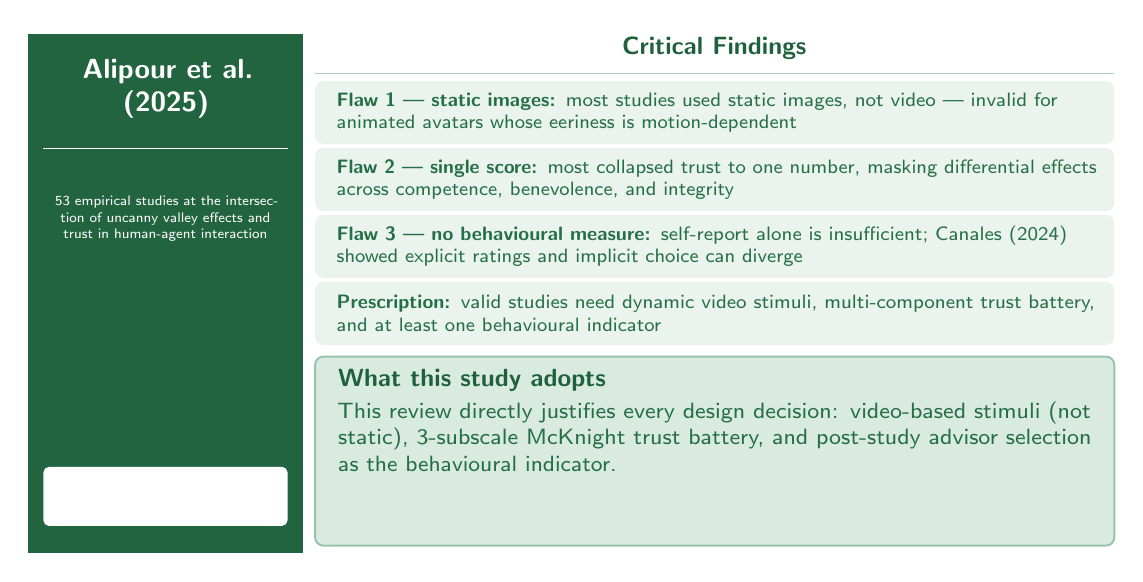
\begin{tikzpicture}[x=1cm, y=1cm]
\fill[kgreen!72!black] (0.0,0.0) rectangle (3.5,6.6);
\node[font=\normalsize\sffamily\bfseries, text=white, align=center, text width=3.1cm]
  at (1.75,5.9) {Alipour et al.\\(2025)};
\draw[white!30, line width=0.3pt] (0.2,5.15) -- (3.3,5.15);
\node[font=\tiny\sffamily, text=white!85, align=center, text width=3.0cm]
  at (1.75,4.25) {53 empirical studies at the intersection of uncanny valley effects and trust in human-agent interaction};
\fill[white!20, rounded corners=2pt] (0.2,0.35) rectangle (3.3,1.10);
\node[font=\tiny\sffamily\bfseries, text=white, align=center]
  at (1.75,0.72) {Systematic review\\53 studies};
\node[font=\small\sffamily\bfseries\color{kgreen!70!black}] at (8.72,6.42) {Critical Findings};
\draw[kgreen!40, line width=0.3pt] (3.65,6.10) -- (13.8,6.10);
\fill[kgreen!10, rounded corners=3pt] (3.65,5.20) rectangle (13.8,6.00);
\node[font=\scriptsize\sffamily\color{kgreen!80!black}, anchor=west, text width=9.65cm]
  at (3.80,5.60) {\textbf{Flaw 1 --- static images:} most studies used static images, not video --- invalid for animated avatars whose eeriness is motion-dependent};
\fill[kgreen!10, rounded corners=3pt] (3.65,4.35) rectangle (13.8,5.15);
\node[font=\scriptsize\sffamily\color{kgreen!80!black}, anchor=west, text width=9.65cm]
  at (3.80,4.75) {\textbf{Flaw 2 --- single score:} most collapsed trust to one number, masking differential effects across competence, benevolence, and integrity};
\fill[kgreen!10, rounded corners=3pt] (3.65,3.50) rectangle (13.8,4.30);
\node[font=\scriptsize\sffamily\color{kgreen!80!black}, anchor=west, text width=9.65cm]
  at (3.80,3.90) {\textbf{Flaw 3 --- no behavioural measure:} self-report alone is insufficient; Canales (2024) showed explicit ratings and implicit choice can diverge};
\fill[kgreen!10, rounded corners=3pt] (3.65,2.65) rectangle (13.8,3.45);
\node[font=\scriptsize\sffamily\color{kgreen!80!black}, anchor=west, text width=9.65cm]
  at (3.80,3.05) {\textbf{Prescription:} valid studies need dynamic video stimuli, multi-component trust battery, and at least one behavioural indicator};
\fill[kgreen!18, draw=kgreen!50, rounded corners=3pt, line width=0.7pt]
  (3.65,0.1) rectangle (13.8,2.50);
\node[font=\small\sffamily\bfseries\color{kgreen!70!black}, anchor=west]
  at (3.82,2.2) {What this study adopts};
\node[font=\footnotesize\sffamily\color{kgreen!80!black}, anchor=north west, text width=9.65cm]
  at (3.82,2.05) {This review directly justifies every design decision: video-based stimuli (not static), 3-subscale McKnight trust battery, and post-study advisor selection as the behavioural indicator.};
\end{tikzpicture}
\end{center}
\end{frame}

%% ═══════════════════════════════════════════════════════════════════════════
%% Nowak & Biocca 2003
%% ═══════════════════════════════════════════════════════════════════════════
\begin{frame}{Nowak \& Biocca (2003) \textnormal{\normalsize --- Agency, Anthropomorphism, and Social Presence}}
\begin{center}
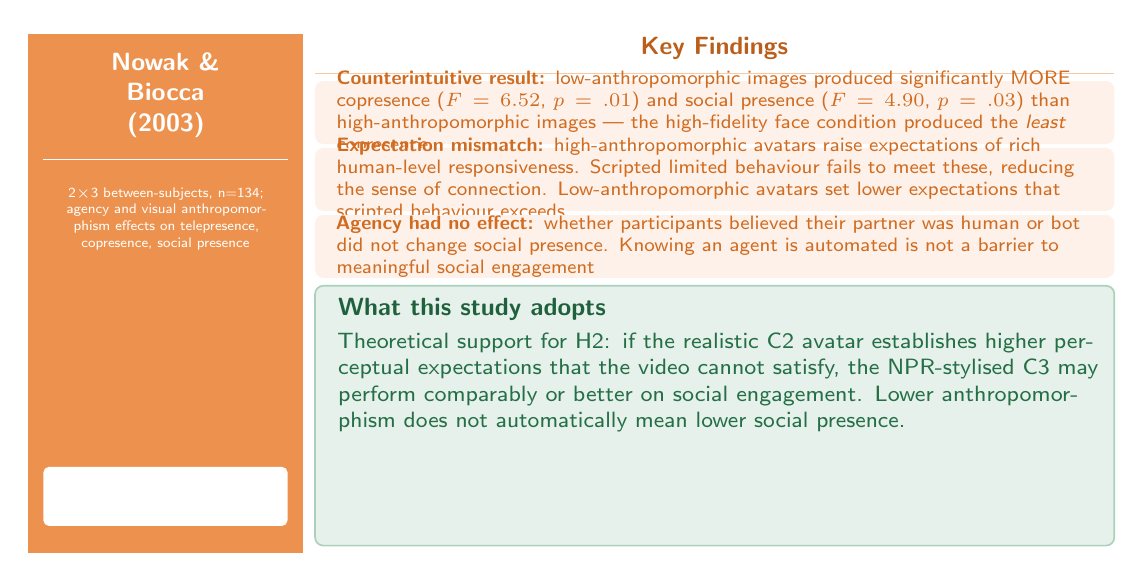
\begin{tikzpicture}[x=1cm, y=1cm]
\fill[korange!80] (0.0,0.0) rectangle (3.5,6.6);
\node[font=\small\sffamily\bfseries, text=white, align=center, text width=3.1cm]
  at (1.75,5.82) {Nowak \&\\Biocca\\(2003)};
\draw[white!30, line width=0.3pt] (0.2,5.00) -- (3.3,5.00);
\node[font=\tiny\sffamily, text=white!85, align=center, text width=3.0cm]
  at (1.75,4.25) {2$\times$3 between-subjects, n=134; agency and visual anthropomorphism effects on telepresence, copresence, social presence};
\fill[white!20, rounded corners=2pt] (0.2,0.35) rectangle (3.3,1.10);
\node[font=\tiny\sffamily\bfseries, text=white, align=center]
  at (1.75,0.72) {Empirical\\n = 134};
\node[font=\small\sffamily\bfseries\color{korange!80!black}] at (8.72,6.42) {Key Findings};
\draw[korange!40, line width=0.3pt] (3.65,6.10) -- (13.8,6.10);
\fill[korange!10, rounded corners=3pt] (3.65,5.20) rectangle (13.8,6.00);
\node[font=\scriptsize\sffamily\color{korange!90!black}, anchor=west, text width=9.65cm]
  at (3.80,5.60) {\textbf{Counterintuitive result:} low-anthropomorphic images produced significantly MORE copresence ($F=6.52$, $p=.01$) and social presence ($F=4.90$, $p=.03$) than high-anthropomorphic images --- the high-fidelity face condition produced the \emph{least} copresence};
\fill[korange!10, rounded corners=3pt] (3.65,4.35) rectangle (13.8,5.15);
\node[font=\scriptsize\sffamily\color{korange!90!black}, anchor=west, text width=9.65cm]
  at (3.80,4.75) {\textbf{Expectation mismatch:} high-anthropomorphic avatars raise expectations of rich human-level responsiveness. Scripted limited behaviour fails to meet these, reducing the sense of connection. Low-anthropomorphic avatars set lower expectations that scripted behaviour exceeds};
\fill[korange!10, rounded corners=3pt] (3.65,3.50) rectangle (13.8,4.30);
\node[font=\scriptsize\sffamily\color{korange!90!black}, anchor=west, text width=9.65cm]
  at (3.80,3.90) {\textbf{Agency had no effect:} whether participants believed their partner was human or bot did not change social presence. Knowing an agent is automated is not a barrier to meaningful social engagement};
\fill[kgreen!12, draw=kgreen!40, rounded corners=3pt, line width=0.6pt]
  (3.65,0.1) rectangle (13.8,3.40);
\node[font=\small\sffamily\bfseries\color{kgreen!70!black}, anchor=west]
  at (3.82,3.1) {What this study adopts};
\node[font=\footnotesize\sffamily\color{kgreen!80!black}, anchor=north west, text width=9.65cm]
  at (3.82,2.92) {Theoretical support for H2: if the realistic C2 avatar establishes higher perceptual expectations that the video cannot satisfy, the NPR-stylised C3 may perform comparably or better on social engagement. Lower anthropomorphism does not automatically mean lower social presence.};
\end{tikzpicture}
\end{center}
\end{frame}

%% ═══════════════════════════════════════════════════════════════════════════
%% Nowak & Rauh 2005
%% ═══════════════════════════════════════════════════════════════════════════
\begin{frame}{Nowak \& Rauh (2005) \textnormal{\normalsize --- Avatar Appearance and Online Social Perceptions}}
\begin{center}
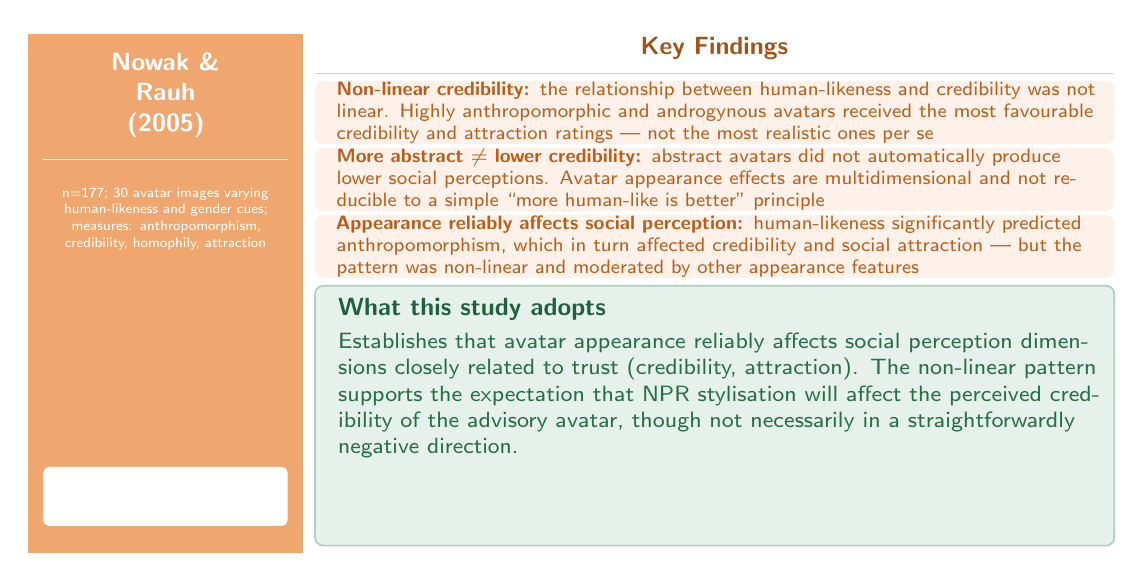
\begin{tikzpicture}[x=1cm, y=1cm]
\fill[korange!65] (0.0,0.0) rectangle (3.5,6.6);
\node[font=\small\sffamily\bfseries, text=white, align=center, text width=3.1cm]
  at (1.75,5.82) {Nowak \&\\Rauh\\(2005)};
\draw[white!30, line width=0.3pt] (0.2,5.00) -- (3.3,5.00);
\node[font=\tiny\sffamily, text=white!85, align=center, text width=3.0cm]
  at (1.75,4.25) {n=177; 30 avatar images varying human-likeness and gender cues; measures: anthropomorphism, credibility, homophily, attraction};
\fill[white!20, rounded corners=2pt] (0.2,0.35) rectangle (3.3,1.10);
\node[font=\tiny\sffamily\bfseries, text=white, align=center]
  at (1.75,0.72) {Empirical\\n = 177};
\node[font=\small\sffamily\bfseries\color{korange!70!black}] at (8.72,6.42) {Key Findings};
\draw[korange!40, line width=0.3pt] (3.65,6.10) -- (13.8,6.10);
\fill[korange!10, rounded corners=3pt] (3.65,5.20) rectangle (13.8,6.00);
\node[font=\scriptsize\sffamily\color{korange!80!black}, anchor=west, text width=9.65cm]
  at (3.80,5.60) {\textbf{Non-linear credibility:} the relationship between human-likeness and credibility was not linear. Highly anthropomorphic and androgynous avatars received the most favourable credibility and attraction ratings --- not the most realistic ones per se};
\fill[korange!10, rounded corners=3pt] (3.65,4.35) rectangle (13.8,5.15);
\node[font=\scriptsize\sffamily\color{korange!80!black}, anchor=west, text width=9.65cm]
  at (3.80,4.75) {\textbf{More abstract $\neq$ lower credibility:} abstract avatars did not automatically produce lower social perceptions. Avatar appearance effects are multidimensional and not reducible to a simple ``more human-like is better'' principle};
\fill[korange!10, rounded corners=3pt] (3.65,3.50) rectangle (13.8,4.30);
\node[font=\scriptsize\sffamily\color{korange!80!black}, anchor=west, text width=9.65cm]
  at (3.80,3.90) {\textbf{Appearance reliably affects social perception:} human-likeness significantly predicted anthropomorphism, which in turn affected credibility and social attraction --- but the pattern was non-linear and moderated by other appearance features};
\fill[kgreen!12, draw=kgreen!40, rounded corners=3pt, line width=0.6pt]
  (3.65,0.1) rectangle (13.8,3.40);
\node[font=\small\sffamily\bfseries\color{kgreen!70!black}, anchor=west]
  at (3.82,3.1) {What this study adopts};
\node[font=\footnotesize\sffamily\color{kgreen!80!black}, anchor=north west, text width=9.65cm]
  at (3.82,2.92) {Establishes that avatar appearance reliably affects social perception dimensions closely related to trust (credibility, attraction). The non-linear pattern supports the expectation that NPR stylisation will affect the perceived credibility of the advisory avatar, though not necessarily in a straightforwardly negative direction.};
\end{tikzpicture}
\end{center}
\end{frame}

%% ═══════════════════════════════════════════════════════════════════════════
%% Weidner et al. 2023
%% ═══════════════════════════════════════════════════════════════════════════
\begin{frame}{Weidner et al. (2023) \textnormal{\normalsize --- Systematic Review of Avatars in AR and VR}}
\begin{center}
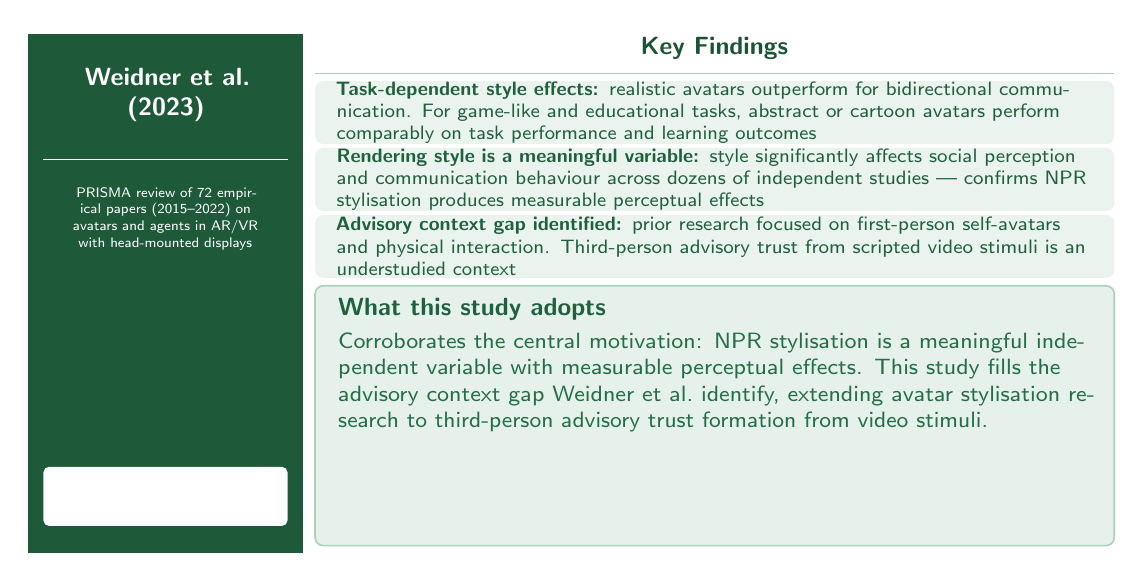
\begin{tikzpicture}[x=1cm, y=1cm]
\fill[kgreen!65!black] (0.0,0.0) rectangle (3.5,6.6);
\node[font=\small\sffamily\bfseries, text=white, align=center, text width=3.1cm]
  at (1.75,5.82) {Weidner et al.\\(2023)};
\draw[white!30, line width=0.3pt] (0.2,5.00) -- (3.3,5.00);
\node[font=\tiny\sffamily, text=white!85, align=center, text width=3.0cm]
  at (1.75,4.25) {PRISMA review of 72 empirical papers (2015--2022) on avatars and agents in AR/VR with head-mounted displays};
\fill[white!20, rounded corners=2pt] (0.2,0.35) rectangle (3.3,1.10);
\node[font=\tiny\sffamily\bfseries, text=white, align=center]
  at (1.75,0.72) {Systematic review\\72 studies};
\node[font=\small\sffamily\bfseries\color{kgreen!60!black}] at (8.72,6.42) {Key Findings};
\draw[kgreen!40, line width=0.3pt] (3.65,6.10) -- (13.8,6.10);
\fill[kgreen!10, rounded corners=3pt] (3.65,5.20) rectangle (13.8,6.00);
\node[font=\scriptsize\sffamily\color{kgreen!70!black}, anchor=west, text width=9.65cm]
  at (3.80,5.60) {\textbf{Task-dependent style effects:} realistic avatars outperform for bidirectional communication. For game-like and educational tasks, abstract or cartoon avatars perform comparably on task performance and learning outcomes};
\fill[kgreen!10, rounded corners=3pt] (3.65,4.35) rectangle (13.8,5.15);
\node[font=\scriptsize\sffamily\color{kgreen!70!black}, anchor=west, text width=9.65cm]
  at (3.80,4.75) {\textbf{Rendering style is a meaningful variable:} style significantly affects social perception and communication behaviour across dozens of independent studies --- confirms NPR stylisation produces measurable perceptual effects};
\fill[kgreen!10, rounded corners=3pt] (3.65,3.50) rectangle (13.8,4.30);
\node[font=\scriptsize\sffamily\color{kgreen!70!black}, anchor=west, text width=9.65cm]
  at (3.80,3.90) {\textbf{Advisory context gap identified:} prior research focused on first-person self-avatars and physical interaction. Third-person advisory trust from scripted video stimuli is an understudied context};
\fill[kgreen!12, draw=kgreen!40, rounded corners=3pt, line width=0.6pt]
  (3.65,0.1) rectangle (13.8,3.40);
\node[font=\small\sffamily\bfseries\color{kgreen!70!black}, anchor=west]
  at (3.82,3.1) {What this study adopts};
\node[font=\footnotesize\sffamily\color{kgreen!80!black}, anchor=north west, text width=9.65cm]
  at (3.82,2.92) {Corroborates the central motivation: NPR stylisation is a meaningful independent variable with measurable perceptual effects. This study fills the advisory context gap Weidner et al.\ identify, extending avatar stylisation research to third-person advisory trust formation from video stimuli.};
\end{tikzpicture}
\end{center}
\end{frame}

%% ═══════════════════════════════════════════════════════════════════════════
%% Kuffner dos Anjos & Pereira 2024
%% ═══════════════════════════════════════════════════════════════════════════
\begin{frame}{Kuffner dos Anjos \& Pereira (2024) \textnormal{\normalsize --- Realism and Self-Embodied Avatars}}
\begin{center}
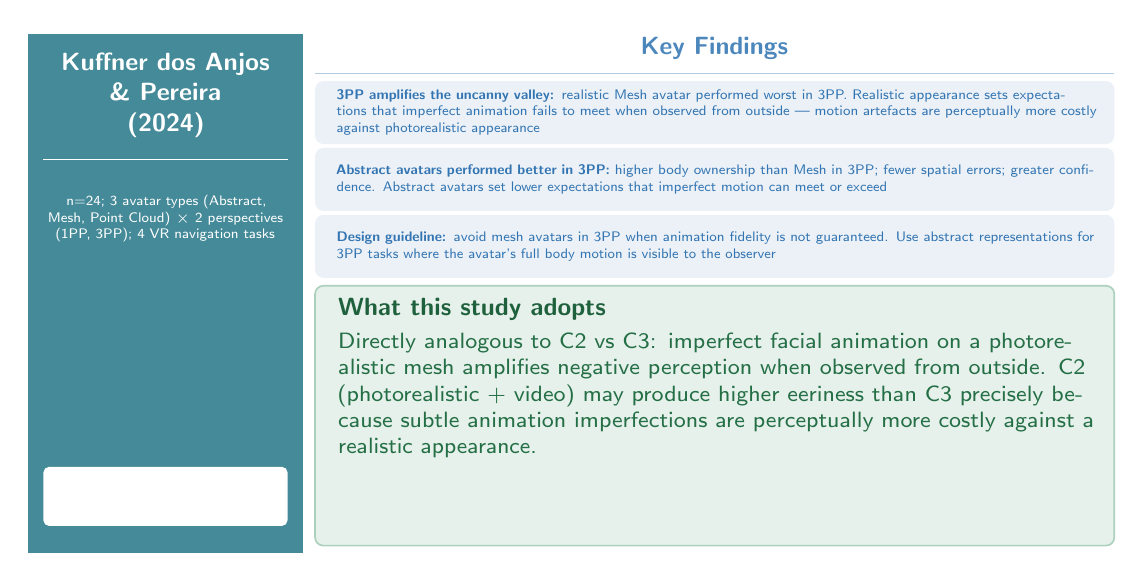
\begin{tikzpicture}[x=1cm, y=1cm]
\fill[kblue!55!kgreen!80] (0.0,0.0) rectangle (3.5,6.6);
\node[font=\small\sffamily\bfseries, text=white, align=center, text width=3.1cm]
  at (1.75,5.82) {Kuffner dos Anjos\\\& Pereira\\(2024)};
\draw[white!30, line width=0.3pt] (0.2,5.00) -- (3.3,5.00);
\node[font=\tiny\sffamily, text=white!85, align=center, text width=3.0cm]
  at (1.75,4.25) {n=24; 3 avatar types (Abstract, Mesh, Point Cloud) $\times$ 2 perspectives (1PP, 3PP); 4 VR navigation tasks};
\fill[white!20, rounded corners=2pt] (0.2,0.35) rectangle (3.3,1.10);
\node[font=\tiny\sffamily\bfseries, text=white, align=center]
  at (1.75,0.72) {Empirical, VR\\n = 24};
\node[font=\small\sffamily\bfseries\color{kblue!70}] at (8.72,6.42) {Key Findings};
\draw[kblue!30, line width=0.3pt] (3.65,6.10) -- (13.8,6.10);
\fill[kblue!8, rounded corners=3pt] (3.65,5.20) rectangle (13.8,6.00);
\node[font=\tiny\sffamily\color{kblue!80}, anchor=west, text width=9.65cm]
  at (3.80,5.60) {\textbf{3PP amplifies the uncanny valley:} realistic Mesh avatar performed worst in 3PP. Realistic appearance sets expectations that imperfect animation fails to meet when observed from outside --- motion artefacts are perceptually more costly against photorealistic appearance};
\fill[kblue!8, rounded corners=3pt] (3.65,4.35) rectangle (13.8,5.15);
\node[font=\tiny\sffamily\color{kblue!80}, anchor=west, text width=9.65cm]
  at (3.80,4.75) {\textbf{Abstract avatars performed better in 3PP:} higher body ownership than Mesh in 3PP; fewer spatial errors; greater confidence. Abstract avatars set lower expectations that imperfect motion can meet or exceed};
\fill[kblue!8, rounded corners=3pt] (3.65,3.50) rectangle (13.8,4.30);
\node[font=\tiny\sffamily\color{kblue!80}, anchor=west, text width=9.65cm]
  at (3.80,3.90) {\textbf{Design guideline:} avoid mesh avatars in 3PP when animation fidelity is not guaranteed. Use abstract representations for 3PP tasks where the avatar's full body motion is visible to the observer};
\fill[kgreen!12, draw=kgreen!40, rounded corners=3pt, line width=0.6pt]
  (3.65,0.1) rectangle (13.8,3.40);
\node[font=\small\sffamily\bfseries\color{kgreen!70!black}, anchor=west]
  at (3.82,3.1) {What this study adopts};
\node[font=\footnotesize\sffamily\color{kgreen!80!black}, anchor=north west, text width=9.65cm]
  at (3.82,2.92) {Directly analogous to C2 vs C3: imperfect facial animation on a photorealistic mesh amplifies negative perception when observed from outside. C2 (photorealistic + video) may produce higher eeriness than C3 precisely because subtle animation imperfections are perceptually more costly against a realistic appearance.};
\end{tikzpicture}
\end{center}
\end{frame}

%% ═══════════════════════════════════════════════════════════════════════════
%% Alimardani et al. 2024
%% ═══════════════════════════════════════════════════════════════════════════
\begin{frame}{Alimardani et al. (2024) \textnormal{\normalsize --- Appearance, Voice, and Trust in Virtual Agent Collaboration}}
\begin{center}
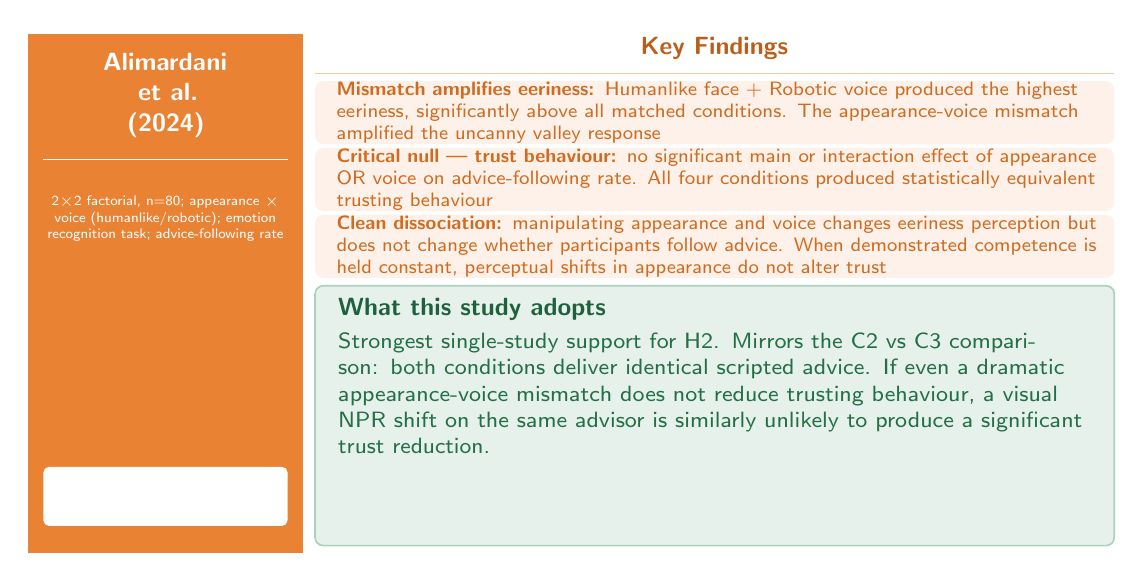
\begin{tikzpicture}[x=1cm, y=1cm]
\fill[korange!92] (0.0,0.0) rectangle (3.5,6.6);
\node[font=\small\sffamily\bfseries, text=white, align=center, text width=3.1cm]
  at (1.75,5.82) {Alimardani\\et al.\\(2024)};
\draw[white!30, line width=0.3pt] (0.2,5.00) -- (3.3,5.00);
\node[font=\tiny\sffamily, text=white!85, align=center, text width=3.0cm]
  at (1.75,4.25) {2$\times$2 factorial, n=80; appearance $\times$ voice (humanlike/robotic); emotion recognition task; advice-following rate};
\fill[white!20, rounded corners=2pt] (0.2,0.35) rectangle (3.3,1.10);
\node[font=\tiny\sffamily\bfseries, text=white, align=center]
  at (1.75,0.72) {Empirical\\n = 80};
\node[font=\small\sffamily\bfseries\color{korange!80!black}] at (8.72,6.42) {Key Findings};
\draw[korange!40, line width=0.3pt] (3.65,6.10) -- (13.8,6.10);
\fill[korange!10, rounded corners=3pt] (3.65,5.20) rectangle (13.8,6.00);
\node[font=\scriptsize\sffamily\color{korange!90!black}, anchor=west, text width=9.65cm]
  at (3.80,5.60) {\textbf{Mismatch amplifies eeriness:} Humanlike face + Robotic voice produced the highest eeriness, significantly above all matched conditions. The appearance-voice mismatch amplified the uncanny valley response};
\fill[korange!10, rounded corners=3pt] (3.65,4.35) rectangle (13.8,5.15);
\node[font=\scriptsize\sffamily\color{korange!90!black}, anchor=west, text width=9.65cm]
  at (3.80,4.75) {\textbf{Critical null --- trust behaviour:} no significant main or interaction effect of appearance OR voice on advice-following rate. All four conditions produced statistically equivalent trusting behaviour};
\fill[korange!10, rounded corners=3pt] (3.65,3.50) rectangle (13.8,4.30);
\node[font=\scriptsize\sffamily\color{korange!90!black}, anchor=west, text width=9.65cm]
  at (3.80,3.90) {\textbf{Clean dissociation:} manipulating appearance and voice changes eeriness perception but does not change whether participants follow advice. When demonstrated competence is held constant, perceptual shifts in appearance do not alter trust};
\fill[kgreen!12, draw=kgreen!40, rounded corners=3pt, line width=0.6pt]
  (3.65,0.1) rectangle (13.8,3.40);
\node[font=\small\sffamily\bfseries\color{kgreen!70!black}, anchor=west]
  at (3.82,3.1) {What this study adopts};
\node[font=\footnotesize\sffamily\color{kgreen!80!black}, anchor=north west, text width=9.65cm]
  at (3.82,2.92) {Strongest single-study support for H2. Mirrors the C2 vs C3 comparison: both conditions deliver identical scripted advice. If even a dramatic appearance-voice mismatch does not reduce trusting behaviour, a visual NPR shift on the same advisor is similarly unlikely to produce a significant trust reduction.};
\end{tikzpicture}
\end{center}
\end{frame}

%% ═══════════════════════════════════════════════════════════════════════════
%% Dubosc et al. 2025
%% ═══════════════════════════════════════════════════════════════════════════
\begin{frame}{Dubosc et al. (2025) \textnormal{\normalsize --- Avatar Stylisation and Facial Expression Intensity}}
\begin{center}
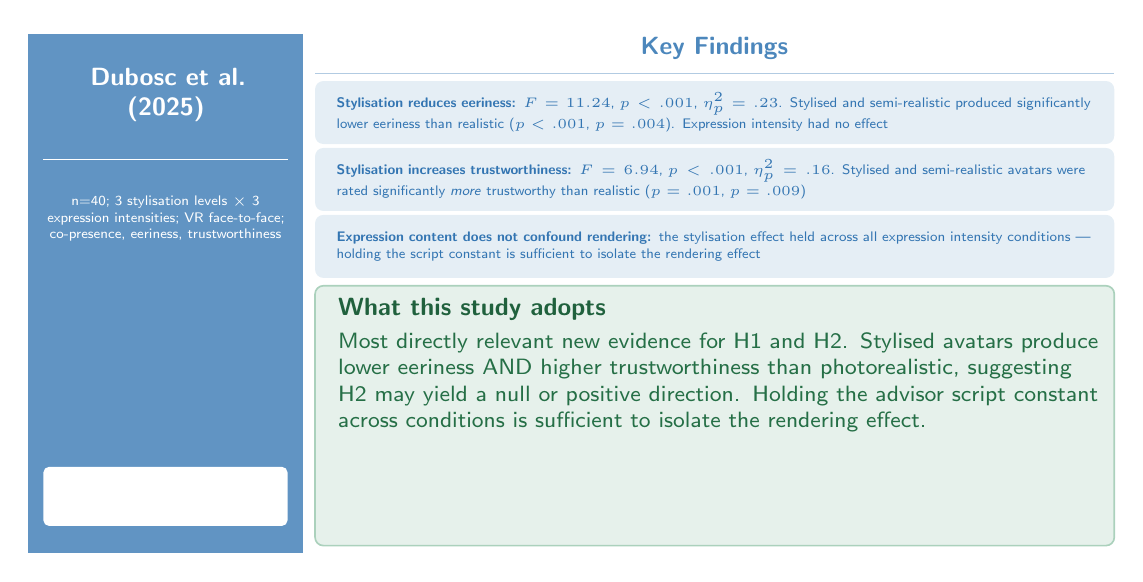
\begin{tikzpicture}[x=1cm, y=1cm]
\fill[kblue!62] (0.0,0.0) rectangle (3.5,6.6);
\node[font=\small\sffamily\bfseries, text=white, align=center, text width=3.1cm]
  at (1.75,5.82) {Dubosc et al.\\(2025)};
\draw[white!30, line width=0.3pt] (0.2,5.00) -- (3.3,5.00);
\node[font=\tiny\sffamily, text=white!85, align=center, text width=3.0cm]
  at (1.75,4.25) {n=40; 3 stylisation levels $\times$ 3 expression intensities; VR face-to-face; co-presence, eeriness, trustworthiness};
\fill[white!20, rounded corners=2pt] (0.2,0.35) rectangle (3.3,1.10);
\node[font=\tiny\sffamily\bfseries, text=white, align=center]
  at (1.75,0.72) {Empirical, VR\\n = 40};
\node[font=\small\sffamily\bfseries\color{kblue!70}] at (8.72,6.42) {Key Findings};
\draw[kblue!30, line width=0.3pt] (3.65,6.10) -- (13.8,6.10);
\fill[kblue!10, rounded corners=3pt] (3.65,5.20) rectangle (13.8,6.00);
\node[font=\tiny\sffamily\color{kblue!80}, anchor=west, text width=9.65cm]
  at (3.80,5.60) {\textbf{Stylisation reduces eeriness:} $F=11.24$, $p<.001$, $\eta^2_p=.23$. Stylised and semi-realistic produced significantly lower eeriness than realistic ($p<.001$, $p=.004$). Expression intensity had no effect};
\fill[kblue!10, rounded corners=3pt] (3.65,4.35) rectangle (13.8,5.15);
\node[font=\tiny\sffamily\color{kblue!80}, anchor=west, text width=9.65cm]
  at (3.80,4.75) {\textbf{Stylisation increases trustworthiness:} $F=6.94$, $p<.001$, $\eta^2_p=.16$. Stylised and semi-realistic avatars were rated significantly \emph{more} trustworthy than realistic ($p=.001$, $p=.009$)};
\fill[kblue!10, rounded corners=3pt] (3.65,3.50) rectangle (13.8,4.30);
\node[font=\tiny\sffamily\color{kblue!80}, anchor=west, text width=9.65cm]
  at (3.80,3.90) {\textbf{Expression content does not confound rendering:} the stylisation effect held across all expression intensity conditions --- holding the script constant is sufficient to isolate the rendering effect};
\fill[kgreen!12, draw=kgreen!40, rounded corners=3pt, line width=0.6pt]
  (3.65,0.1) rectangle (13.8,3.40);
\node[font=\small\sffamily\bfseries\color{kgreen!70!black}, anchor=west]
  at (3.82,3.1) {What this study adopts};
\node[font=\footnotesize\sffamily\color{kgreen!80!black}, anchor=north west, text width=9.65cm]
  at (3.82,2.92) {Most directly relevant new evidence for H1 and H2. Stylised avatars produce lower eeriness AND higher trustworthiness than photorealistic, suggesting H2 may yield a null or positive direction. Holding the advisor script constant across conditions is sufficient to isolate the rendering effect.};
\end{tikzpicture}
\end{center}
\end{frame}

%% ═══════════════════════════════════════════════════════════════════════════
%% Tao et al. 2025
%% ═══════════════════════════════════════════════════════════════════════════
\begin{frame}{Tao et al. (2025) \textnormal{\normalsize --- Network Meta-Analysis of Avatar Realism}}
\begin{center}
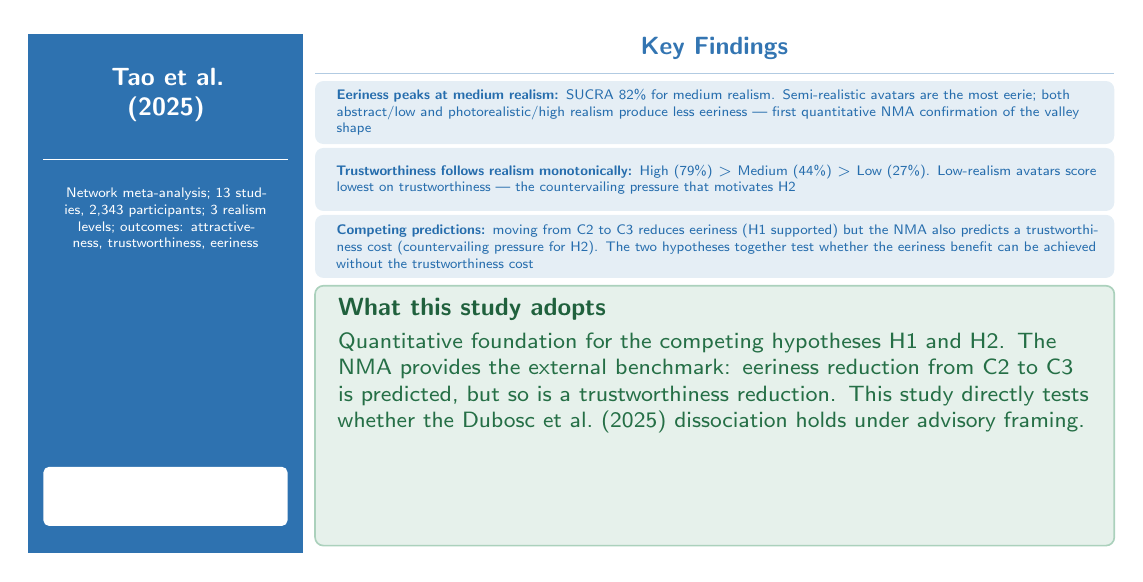
\begin{tikzpicture}[x=1cm, y=1cm]
\fill[kblue!82] (0.0,0.0) rectangle (3.5,6.6);
\node[font=\small\sffamily\bfseries, text=white, align=center, text width=3.1cm]
  at (1.75,5.82) {Tao et al.\\(2025)};
\draw[white!30, line width=0.3pt] (0.2,5.00) -- (3.3,5.00);
\node[font=\tiny\sffamily, text=white!85, align=center, text width=3.0cm]
  at (1.75,4.25) {Network meta-analysis; 13 studies, 2,343 participants; 3 realism levels; outcomes: attractiveness, trustworthiness, eeriness};
\fill[white!20, rounded corners=2pt] (0.2,0.35) rectangle (3.3,1.10);
\node[font=\tiny\sffamily\bfseries, text=white, align=center]
  at (1.75,0.72) {Network meta-analysis\\n = 2{,}343};
\node[font=\small\sffamily\bfseries\color{kblue!80}] at (8.72,6.42) {Key Findings};
\draw[kblue!30, line width=0.3pt] (3.65,6.10) -- (13.8,6.10);
\fill[kblue!10, rounded corners=3pt] (3.65,5.20) rectangle (13.8,6.00);
\node[font=\tiny\sffamily\color{kblue!85}, anchor=west, text width=9.65cm]
  at (3.80,5.60) {\textbf{Eeriness peaks at medium realism:} SUCRA 82\% for medium realism. Semi-realistic avatars are the most eerie; both abstract/low and photorealistic/high realism produce less eeriness --- first quantitative NMA confirmation of the valley shape};
\fill[kblue!10, rounded corners=3pt] (3.65,4.35) rectangle (13.8,5.15);
\node[font=\tiny\sffamily\color{kblue!85}, anchor=west, text width=9.65cm]
  at (3.80,4.75) {\textbf{Trustworthiness follows realism monotonically:} High (79\%) $>$ Medium (44\%) $>$ Low (27\%). Low-realism avatars score lowest on trustworthiness --- the countervailing pressure that motivates H2};
\fill[kblue!10, rounded corners=3pt] (3.65,3.50) rectangle (13.8,4.30);
\node[font=\tiny\sffamily\color{kblue!85}, anchor=west, text width=9.65cm]
  at (3.80,3.90) {\textbf{Competing predictions:} moving from C2 to C3 reduces eeriness (H1 supported) but the NMA also predicts a trustworthiness cost (countervailing pressure for H2). The two hypotheses together test whether the eeriness benefit can be achieved without the trustworthiness cost};
\fill[kgreen!12, draw=kgreen!40, rounded corners=3pt, line width=0.6pt]
  (3.65,0.1) rectangle (13.8,3.40);
\node[font=\small\sffamily\bfseries\color{kgreen!70!black}, anchor=west]
  at (3.82,3.1) {What this study adopts};
\node[font=\footnotesize\sffamily\color{kgreen!80!black}, anchor=north west, text width=9.65cm]
  at (3.82,2.92) {Quantitative foundation for the competing hypotheses H1 and H2. The NMA provides the external benchmark: eeriness reduction from C2 to C3 is predicted, but so is a trustworthiness reduction. This study directly tests whether the Dubosc et al.\ (2025) dissociation holds under advisory framing.};
\end{tikzpicture}
\end{center}
\end{frame}

%% ═══════════════════════════════════════════════════════════════════════════
%% Cihodaru-Stefanache & Podina 2025
%% ═══════════════════════════════════════════════════════════════════════════
\begin{frame}{Cihodaru-\c{S}tefanache \& Podina (2025) \textnormal{\normalsize --- Uncanny Valley in Embodied Conversational Agents}}
\begin{center}
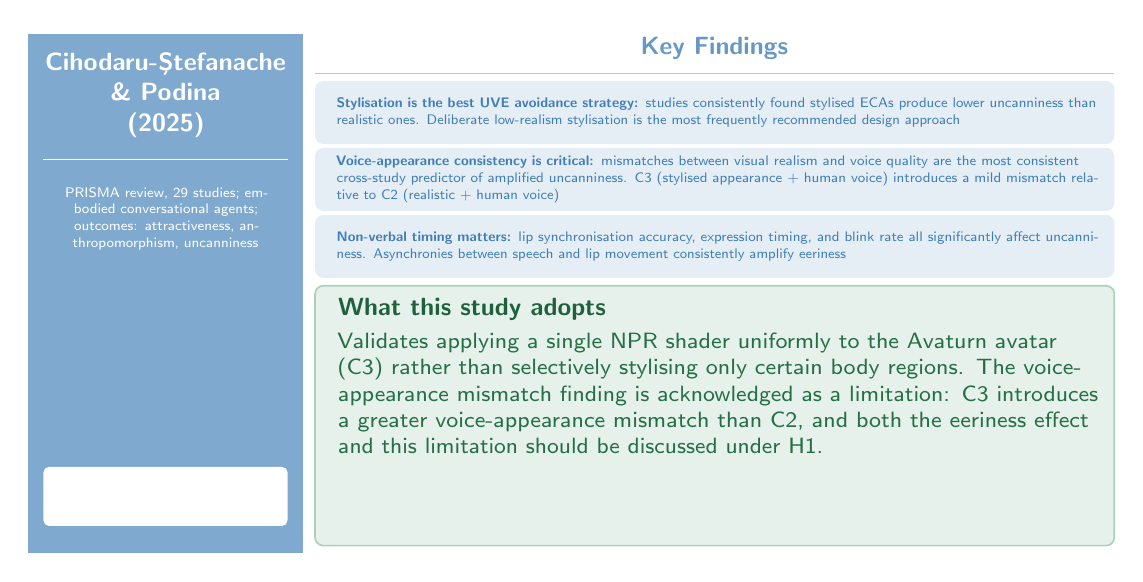
\begin{tikzpicture}[x=1cm, y=1cm]
\fill[kblue!50] (0.0,0.0) rectangle (3.5,6.6);
\node[font=\small\sffamily\bfseries, text=white, align=center, text width=3.1cm]
  at (1.75,5.82) {Cihodaru-\c{S}tefanache\\\& Podina\\(2025)};
\draw[white!30, line width=0.3pt] (0.2,5.00) -- (3.3,5.00);
\node[font=\tiny\sffamily, text=white!85, align=center, text width=3.0cm]
  at (1.75,4.25) {PRISMA review, 29 studies; embodied conversational agents; outcomes: attractiveness, anthropomorphism, uncanniness};
\fill[white!20, rounded corners=2pt] (0.2,0.35) rectangle (3.3,1.10);
\node[font=\tiny\sffamily\bfseries, text=white, align=center]
  at (1.75,0.72) {Systematic review\\29 studies};
\node[font=\small\sffamily\bfseries\color{kblue!60}] at (8.72,6.42) {Key Findings};
\draw[kblue!30, line width=0.3pt] (3.65,6.10) -- (13.8,6.10);
\fill[kblue!10, rounded corners=3pt] (3.65,5.20) rectangle (13.8,6.00);
\node[font=\tiny\sffamily\color{kblue!75}, anchor=west, text width=9.65cm]
  at (3.80,5.60) {\textbf{Stylisation is the best UVE avoidance strategy:} studies consistently found stylised ECAs produce lower uncanniness than realistic ones. Deliberate low-realism stylisation is the most frequently recommended design approach};
\fill[kblue!10, rounded corners=3pt] (3.65,4.35) rectangle (13.8,5.15);
\node[font=\tiny\sffamily\color{kblue!75}, anchor=west, text width=9.65cm]
  at (3.80,4.75) {\textbf{Voice-appearance consistency is critical:} mismatches between visual realism and voice quality are the most consistent cross-study predictor of amplified uncanniness. C3 (stylised appearance + human voice) introduces a mild mismatch relative to C2 (realistic + human voice)};
\fill[kblue!10, rounded corners=3pt] (3.65,3.50) rectangle (13.8,4.30);
\node[font=\tiny\sffamily\color{kblue!75}, anchor=west, text width=9.65cm]
  at (3.80,3.90) {\textbf{Non-verbal timing matters:} lip synchronisation accuracy, expression timing, and blink rate all significantly affect uncanniness. Asynchronies between speech and lip movement consistently amplify eeriness};
\fill[kgreen!12, draw=kgreen!40, rounded corners=3pt, line width=0.6pt]
  (3.65,0.1) rectangle (13.8,3.40);
\node[font=\small\sffamily\bfseries\color{kgreen!70!black}, anchor=west]
  at (3.82,3.1) {What this study adopts};
\node[font=\footnotesize\sffamily\color{kgreen!80!black}, anchor=north west, text width=9.65cm]
  at (3.82,2.92) {Validates applying a single NPR shader uniformly to the Avaturn avatar (C3) rather than selectively stylising only certain body regions. The voice-appearance mismatch finding is acknowledged as a limitation: C3 introduces a greater voice-appearance mismatch than C2, and both the eeriness effect and this limitation should be discussed under H1.};
\end{tikzpicture}
\end{center}
\end{frame}

\begin{frame}{Wallraven et al. (2008) \textnormal{\normalsize --- Evaluating the Perceptual Realism of Animated Facial Expressions}}
\begin{center}
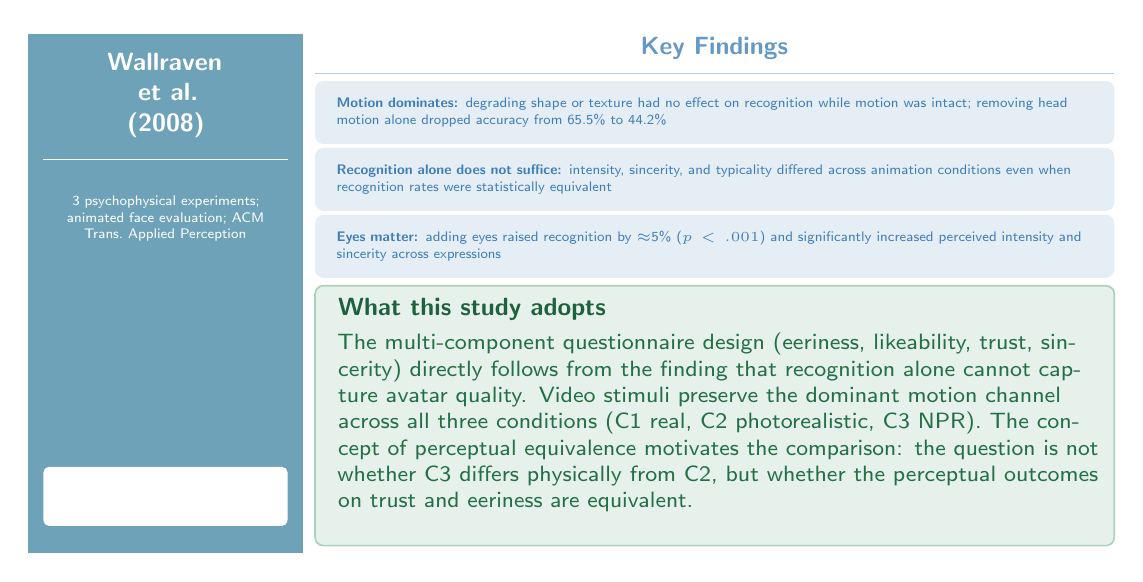
\begin{tikzpicture}[x=1cm, y=1cm]
\fill[kblue!70!kgreen!60] (0.0,0.0) rectangle (3.5,6.6);
\node[font=\small\sffamily\bfseries, text=white, align=center, text width=3.1cm]
  at (1.75,5.82) {Wallraven\\et al.\\(2008)};
\draw[white!30, line width=0.3pt] (0.2,5.00) -- (3.3,5.00);
\node[font=\tiny\sffamily, text=white!85, align=center, text width=3.0cm]
  at (1.75,4.25) {3 psychophysical experiments; animated face evaluation; ACM Trans.\ Applied Perception};
\fill[white!20, rounded corners=2pt] (0.2,0.35) rectangle (3.3,1.10);
\node[font=\tiny\sffamily\bfseries, text=white, align=center]
  at (1.75,0.72) {Psychophysics\\$n = 12$ per experiment};
\node[font=\small\sffamily\bfseries\color{kblue!60}] at (8.72,6.42) {Key Findings};
\draw[kblue!30, line width=0.3pt] (3.65,6.10) -- (13.8,6.10);
\fill[kblue!10, rounded corners=3pt] (3.65,5.20) rectangle (13.8,6.00);
\node[font=\tiny\sffamily\color{kblue!75}, anchor=west, text width=9.65cm]
  at (3.80,5.60) {\textbf{Motion dominates:} degrading shape or texture had no effect on recognition while motion was intact; removing head motion alone dropped accuracy from 65.5\% to 44.2\%};
\fill[kblue!10, rounded corners=3pt] (3.65,4.35) rectangle (13.8,5.15);
\node[font=\tiny\sffamily\color{kblue!75}, anchor=west, text width=9.65cm]
  at (3.80,4.75) {\textbf{Recognition alone does not suffice:} intensity, sincerity, and typicality differed across animation conditions even when recognition rates were statistically equivalent};
\fill[kblue!10, rounded corners=3pt] (3.65,3.50) rectangle (13.8,4.30);
\node[font=\tiny\sffamily\color{kblue!75}, anchor=west, text width=9.65cm]
  at (3.80,3.90) {\textbf{Eyes matter:} adding eyes raised recognition by ${\approx}$5\% ($p < .001$) and significantly increased perceived intensity and sincerity across expressions};
\fill[kgreen!12, draw=kgreen!40, rounded corners=3pt, line width=0.6pt]
  (3.65,0.1) rectangle (13.8,3.40);
\node[font=\small\sffamily\bfseries\color{kgreen!70!black}, anchor=west]
  at (3.82,3.1) {What this study adopts};
\node[font=\footnotesize\sffamily\color{kgreen!80!black}, anchor=north west, text width=9.65cm]
  at (3.82,2.92) {The multi-component questionnaire design (eeriness, likeability, trust, sincerity) directly follows from the finding that recognition alone cannot capture avatar quality. Video stimuli preserve the dominant motion channel across all three conditions (C1 real, C2 photorealistic, C3 NPR). The concept of perceptual equivalence motivates the comparison: the question is not whether C3 differs physically from C2, but whether the perceptual outcomes on trust and eeriness are equivalent.};
\end{tikzpicture}
\end{center}
\end{frame}

\end{document}
